\section{A Quick Exercise in Visualizing Electromagnetic Waves}

\begin{comment}
This lab is more of a worksheet than it is a lab.  But I've used versions of if in my 132 classes for a while, so I thought it was time to include it here in the lab manual for others as well.  --Matt Trawick, 6/2015

This lab/worksheet is designed to address a specific pedagogical challenge: that students don't have a good mental picture of plane waves.  What's hard is that they are typically represented in books as graphs with E and B as functions of x, so that E appears on the y axis, and B appears on the z axis.  Students don't understand what actually happens when you walk a little bit in the spacial y or z direction.

\end{comment}

\makelabheader %(Space for student name, etc., defined in master.tex)

\vspace{0.1in}
%\textbf{Objective} 
%
%This is a quick worksheet to give you some practice in visualizing and working with electromagnetic plane waves.

\textbf{Activity 1}

An electromagnetic \textbf{PLANE} wave is described by
\begin{align*}
\vec E &= E_{MAX} \cos \left ( kx - \omega t \right ) \hat y\\
\vec B &= B_{MAX} \cos \left ( kx - \omega t \right ) \hat z,
\end{align*}
and has a wavelength of $\lambda =12$ meters.  All $(x,y,z)$ points in this problem are in meters.
\vspace{0.1in}

(a) Draw a sketch of the wave on the axes below, at time $t=0$.
\begin{center}
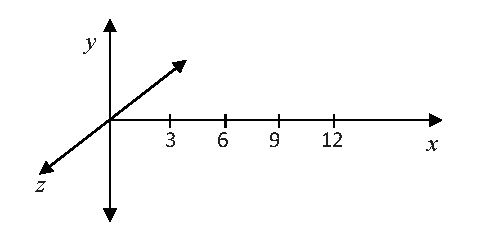
\includegraphics[width=0.4\textwidth]{em_plane_waves/em_waves_axes.eps}
\end{center}

(b) At $t=0$, find both $\vec E$ and $\vec B$ at the points $(0,0,0), (3,0,0), (6,0,0),$ and $(9,0,0)$.  (Your answers are vectors, and should include both \textbf{magnitude} and \textbf{direction}.) 
\vspace{1.0in}

(c) At $t=0$, find both $\vec E$ and $\vec B$ at the points $(0,0,1), (0,1,0), (0,1,1),$ and $(3,1,1)$.  (Remember, it's a plane wave….)
\vspace{1.0in}

(d)  Find the period $T$ and frequency $f$ of the wave.  (Numerical answers, please.)
\vspace{1.0in}

(e)  At $t=10$ nsec, find $\vec E$ and $\vec B$ at the points $(0,0,0), (3,0,0), (6,0,0), (9,0,0),$ and $(3,1,2)$.  
\vspace{1.0in}

